Due to their destructive nature, wildfires are often viewed as something to be avoided at all costs, however wildfires play a crucial role in a variety of ecosystems. In addition to rejuvenating the forest, wildfires can increase soil fertility and remove dead organic material, which decreases the likelihood of a more intense and destructive wildfire in the future \cite{bond_fires_2017}. In most fires, the problem occurs when they spiral out of control, causing unintended damage to wildlife and populations. Global warming and an increase in droughts have led to more frequent intensive wildfires in countries that were not historically prone to them. Throughout the Mediterranean region, countries have become accustomed to this natural destructive cycle and have been able to reduce burned areas since 1980 by improving fire control with Portugal remaining the exception \cite{turco_decreasing_2016, european_commission_joint_research_centre_forest_2021}. Keeping a forest clean is essential for controlling wildfires, and forest maintenance plays a crucial role in doing so. Like in other areas, bringing mechanization into the scope of forestry has greatly improve the productivity, leaving the human component as the bottleneck \cite{parker_robotics_2016}.

According to the \acl{IFR} (\acs{IFR}) report in 2020, the need for robotics is increasing every year  \cite{IFR_robot_report_2020}. Among the many uses of robots, there are healthcare applications, industrial application, agriculture, common households tasks like cleaning as well as dangerous or inaccessible tasks, such as space exploration and mining. It is only natural to assume that robots can play an active role in forestry applications. Although there is not a widespread use of forestry robots, some prototypes were already developed.  Some of these robots are designed to preserve and monitor forests \cite{couceiro_semfire_2019, jelavic_towards_2021, lam_flexible_2011, notomista_slothbot_2019}, while others focus in actively fighting wildfires \cite{noauthor_firefighting_2014, hose_cartridge, hydra}. Furthermore, there are robots specialized in planting, pruning, and harvesting \cite{noauthor_multiscope_nodate, molina_aerial_2017, zhang_rubber-tapping_2019}.

Some of these robots weigh over a ton, have large dimensions, and lack flexibility. Consequently, this movement constraint leads to a slow acquisition of data causing a bottleneck in an engineering project's typical workflow: design, develop, test and repeat, since it results in unnecessary delays between the development and testing phases. This bottleneck can be alleviated by the use of a lightweight and portable system designed to gather data efficiently.

In short, wildfires are important to a healthy ecosystem but they need to be controlled to not damage populations and wildlife. The first step to increasing fire control is to clean the forest of dead organic matter, a task that can be performed by robots. As these robots are heavy, scientists and researchers find it difficult to obtain data directly from them, requiring a light system to record the necessary data to develop and test algorithms.

\section{Objectives}
In this work, we aim to design a rigid multisensory apparatus with an onboard computer to map forests. This apparatus combines multiple sensing technologies, such as 3D \acl{LiDAR} (\acs{LiDAR}), depth cameras, infrared spectroscopy and \acl{IMU} (\acs{IMU}). With this apparatus, we will be able to collect datasets from forest environments, thus supporting forest operations, such as metric-semantic 3D mapping, combustible material identification, and forest cleaning. Aside from designing the apparatus, it is intended to integrate, test, and then compare state-of-the-art 3D mapping techniques based on the ROS middleware.

\section{System Requirements}

In order to create a system able to collect the necessary data while ensuring it complies with the requirements of future projects the MoSCoWW analysis was made and it is presented in Figure \ref{fig: moscoww}.

\begin{figure}[H]
    \centering
    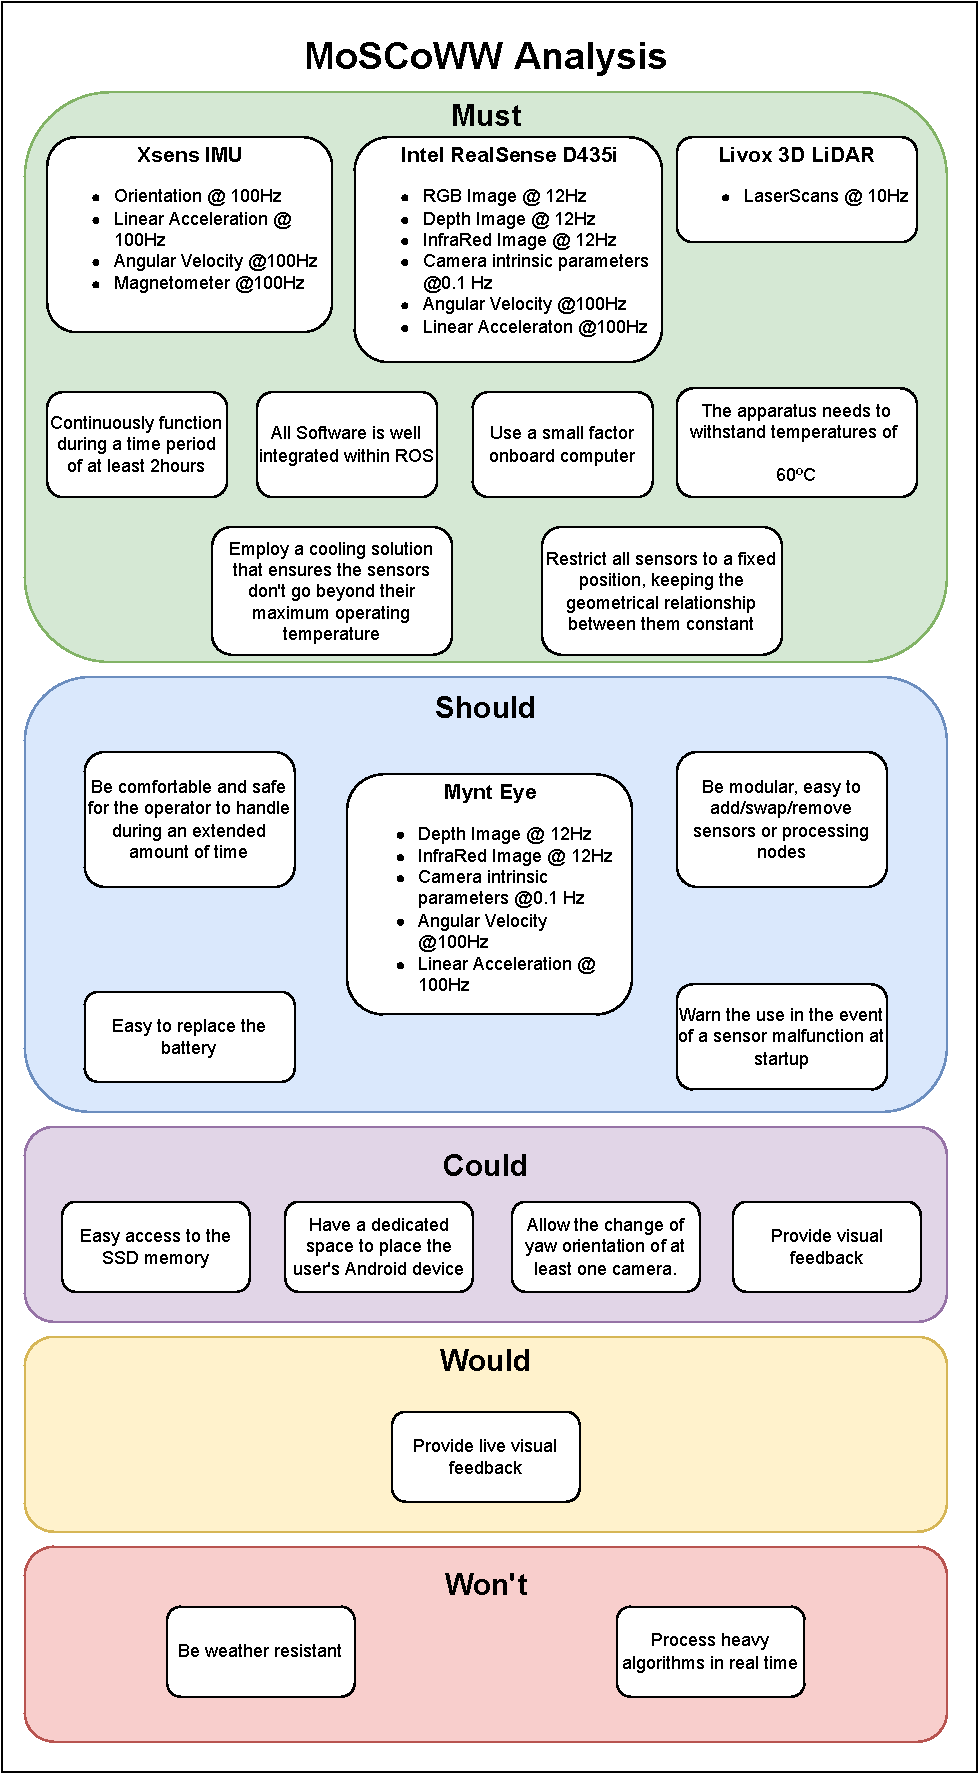
\includegraphics[width=0.875\linewidth]{images/introduction/moscoww_analysis.pdf}
    \caption{MoSCoWW analysis for the project}
    \label{fig: moscoww}
\end{figure}

\section{Dissertation Structure}